\documentclass[a4paper,12pt]{article}
%%%%%%%%%%%%%%%%%%%%%%%%%%%%%%%%%%%%%%%%%%%%%%%%%%%%%%%%%%%%%%%%%%%%%%%%%%%%%%%%%%%%%%%%%%%%%%%%%%%%%%%%%%%%%%%%%%%%%%%%%%%%%%%%%%%%%%%%%%%%%%%%%%%%%%%%%%%%%%%%%%%%%%%%%%%%%%%%%%%%%%%%%%%%%%%%%%%%%%%%%%%%%%%%%%%%%%%%%%%%%%%%%%%%%%%%%%%%%%%%%%%%%%%%%%%%
\usepackage{eurosym}
\usepackage{vmargin}
\usepackage{amsmath}
\usepackage{graphics}
\usepackage{framed}
\usepackage{epsfig}
\usepackage{subfigure}
\usepackage{fancyhdr}

\setcounter{MaxMatrixCols}{10}
%TCIDATA{OutputFilter=LATEX.DLL}
%TCIDATA{Version=5.00.0.2570}
%TCIDATA{<META NAME="SaveForMode"CONTENT="1">}
%TCIDATA{LastRevised=Wednesday, February 23, 201113:24:34}
%TCIDATA{<META NAME="GraphicsSave" CONTENT="32">}
%TCIDATA{Language=American English}

\pagestyle{fancy}
\setmarginsrb{20mm}{0mm}{20mm}{25mm}{12mm}{11mm}{0mm}{11mm}
\lhead{MA4505} \rhead{Kevin O'Brien} \chead{Review Questions for Midterm
and EoS Exam } %\input{tcilatex}

\begin{document}
	\subsection*{Q1. Experimental Design }
	
	% Definitions
	% One Way ANOVA
	% Checking Assumptions
	
	Explain the following terms in the context of experimental design
	\begin{itemize}
		\item[i.] (2 marks) levels of a factor.
		\item[ii.] (2 marks) randomized block design.
	\end{itemize}
	
	%==================================================================%
	\subsection*{Q2. One-Way ANOVA } %4 Marks
	Six analysts each made seven determinations of the paracetamol content of the same batch of tablets.
	The results are shown in the table below. In the last two columns are the sample means and standard deviations for each sample.\\
	\bigskip
	
	\begin{tabular}{|c|ccccccc|c|c|}
		\hline
		Group &  & &  &  &  &  &  & $\bar{X}$& $S_{X}$ \\ \hline
		A & 84.32 & 84.51 & 84.63 & 84.61 & 84.64 & 84.51 & 84.62 & 84.5486 & 0.1209 \\ \hline
		B & 84.24 & 84.25 & 84.41 & 84.13 & 84.00 & 84.30 & 84.02 & 84.1928 & 0.1416 \\ \hline
		C & 84.29 & 84.40 & 84.68 & 84.28 & 84.40 & 84.36 & 84.63 & 84.4342 & 0.1459 \\ \hline
		D & 84.14 & 84.22 & 84.02 & 84.48 & 84.27 & 84.33 & 84.22 & 84.2400 & 0.1583 \\ \hline
		E & 84.50 & 83.88 & 84.49 & 83.91 & 84.11 & 84.06 & 83.99 & 84.1343 & 0.2749 \\ \hline
		F & 84.70 & 84.17 & 84.11 & 84.36 & 84.61 & 83.81 & 84.15 & 84.2729 & 0.3324 \\ \hline
	\end{tabular} 
	

	
	
	\bigskip
	For the aggregrate sample (all 42 observations) the standard deviation is $0.2334$.
	
	\begin{itemize}
		\item[(i)] (5 Marks) Complete the following One Way Analysis of Variance Table.
		\item[(ii)] (1 Marks) Describe what is the purpose of this procedure. include a statement of the null and alternative hypothesis in your answer.
		%	\item[(iii)] (2 Marks) (5 Marks)
	\end{itemize}
	\begin{tabular}{|r|c|c|c|c|c|}
		\hline Source  &\phantom{sp} DF \phantom{sp} & Sum Squares & Mean Square  & \phantom{sp} F \phantom{sp} & p-value  \\ 
		\hline Between-Groups &  &  &  &  & 0.003941 \\ 
		\hline Within-Groups &  &  &  &  &  \\ \hline
		\hline Total &  &  &  &  &  \\ 
		\hline 
	\end{tabular} 
	
\newpage
	
\subsection*{Q3. One Way ANOVA } %4 Marks


\begin{figure}[h!]
	\centering
	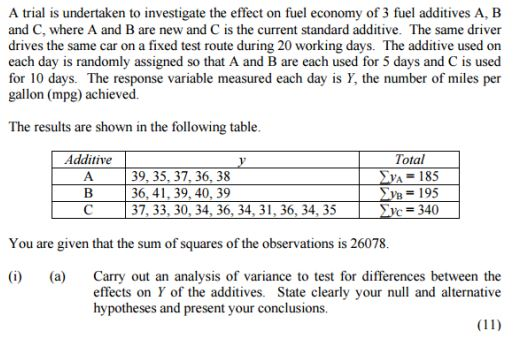
\includegraphics[width=1.0\linewidth]{image/Q23Review}
\end{figure}
\noindent (Important: For MA4505, Disregard the comment about the \textbf{Sum of Square of the Observations}.)\\
You are given the additional piece of information , sufficient to construct ANOVA table

{
	\Large
	\begin{center}
		\begin{tabular}{|c|c|c|c||c|} 
			\hline  & A & B & C & Overall \\ 
			\hline Mean & 37 & 39& 34 &36 \\ 
			\hline Std.Dev &  1.5811 & 1.8708 & 2.2111 & 2.8837 \\
			
			\hline 
		\end{tabular}
	\end{center}
}
The p-value for the Test Statistic is 0.00650

\newpage
\subsection*{Q4. One Way ANOVA }
\begin{figure}[h!]
	\centering
	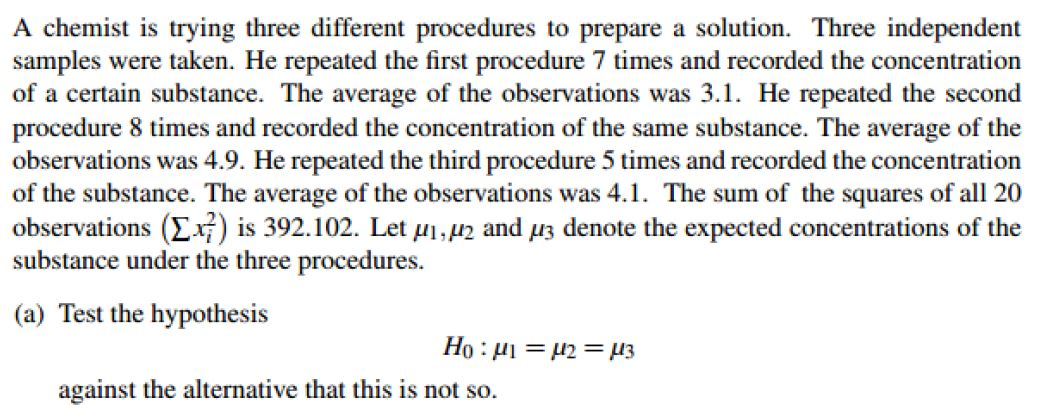
\includegraphics[width=1\linewidth]{image/Q24review1}
	
\end{figure}

\noindent \textbf{Additional Information: }
\begin{itemize}
	\item The Variance of the Response Variable is 3.2. (You can ignore the part about “the sum of squares for all 20 obervations”.)
	\item  Ordinarily you would be given the standard deviation for each sample, and from that, directly compute SSwithin. In this question , use this identity : SStotal = SSbetween + SSwithin.
	\item  You have been given enough information to compute the Overall Mean.
	\item  We may not get around to covering the confidence intervals material in MA4605 2015. It will be retained for possible use in future.
\end{itemize}
\newpage
\subsection*{Q5. One Way ANOVA }
\begin{figure}[h!]
	\centering
	\includegraphics[width=1\linewidth]{image/Q27review1}
	
\end{figure}
\noindent \textbf{Additional Information: }
\begin{itemize}
	\item The variance of the response variable is 831.3695. (\textit{You can ignore now some of the information given in the question}) 
	\item  In this question, use this identity : \textbf{\textit{SStotal = SSbetween + SSwithin}}.
	\item  You have been given enough information to compute the Overall Mean.
	\item  We may not get around to covering the confidence intervals material in MA4605 2015. It will be retained for possible use in future.
\end{itemize}
\newpage
\subsection*{Q6. Two Way ANOVA - No Replicates} %4 Marks

Three varieties of potatoes are being compared for yield. The experiment
was carried out by assigning each variety at random to four of twelve equal size
plots, one being chosen in each of four locations. The following yields in bushels per 
plot resulted:
% A bushel is about 36.4 litres.

\begin{figure}[h!]
	\centering
	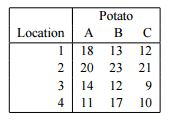
\includegraphics[width=0.4\linewidth]{image/twowayanova-potato}
\end{figure}
\noindent \textbf{Additional Information} 

\begin{itemize}
	\item The variance of the Row means is : $S^2_{R} = 19.037$. 
	\item the variance of the Column means is : $S^2_{C} = 3.0625$.	
	\item Also the overall variance of the 12 observations is $\textrm{Var}(Y) = 21.6363 $. 
\end{itemize}

\noindent \textbf{Exercise:} Complete the Two Way ANOVA table. You are not required to perform any hypothesis testing.
\newpage

\subsection*{Q7. Two Way ANOVA }
Given the following details below, construct the appropriate Two-Way ANOVA Table. \textit{You are not required to do any hypothesis testing.}

\begin{itemize}
	\item There are 2 factors: A and B. A has 2 levels, while Factor B has 3 levels.
	\item There are 54 observations in the experiment.
	\item The variance of the response variable is 174.2075.
	\item The Sum of Squares for Factors A and B are 451  and  2034 respectively.
	\item The Sum of Squares for Error is 5745.
\end{itemize}

\newpage


\subsection*{Q8. Two Way ANOVA (no replicates)}
\begin{figure}[h!]
	\centering
	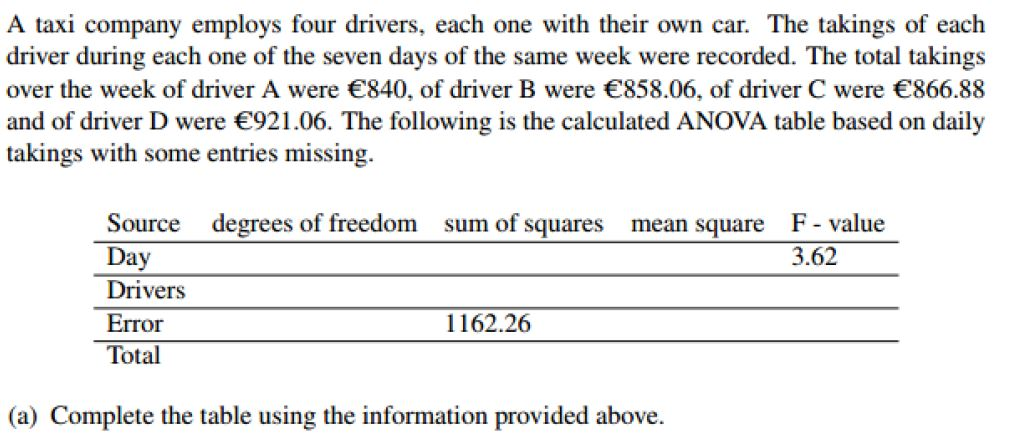
\includegraphics[width=0.9\linewidth]{image/Q26Review1}
	
\end{figure}
\begin{figure}[h!]
	\centering
	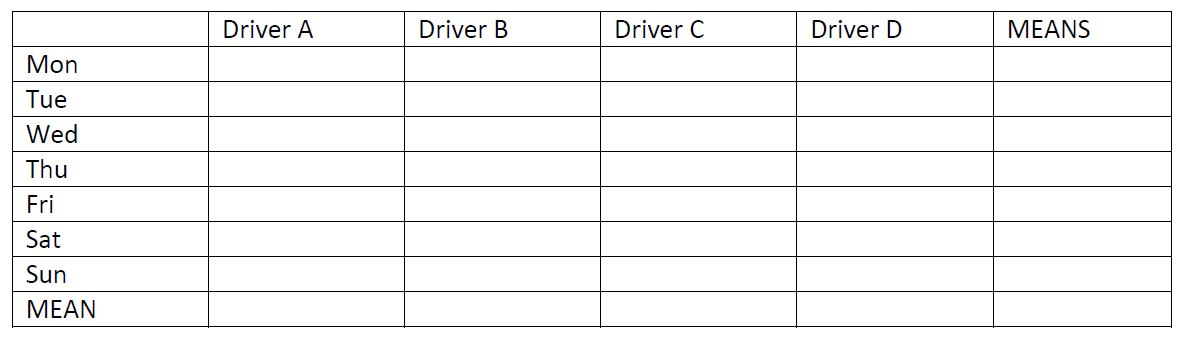
\includegraphics[width=0.9\linewidth]{image/Q26review2}
	
\end{figure}
\begin{figure}[h!]
	\centering
	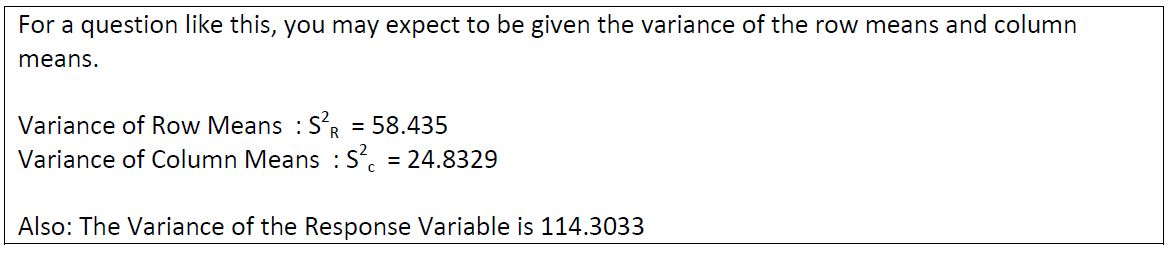
\includegraphics[width=0.9\linewidth]{image/Q26review3}
	
\end{figure}
\newpage

\subsection*{Q9. Two Way ANOVA (no replicates)}
\begin{figure}[h!]
	\centering
	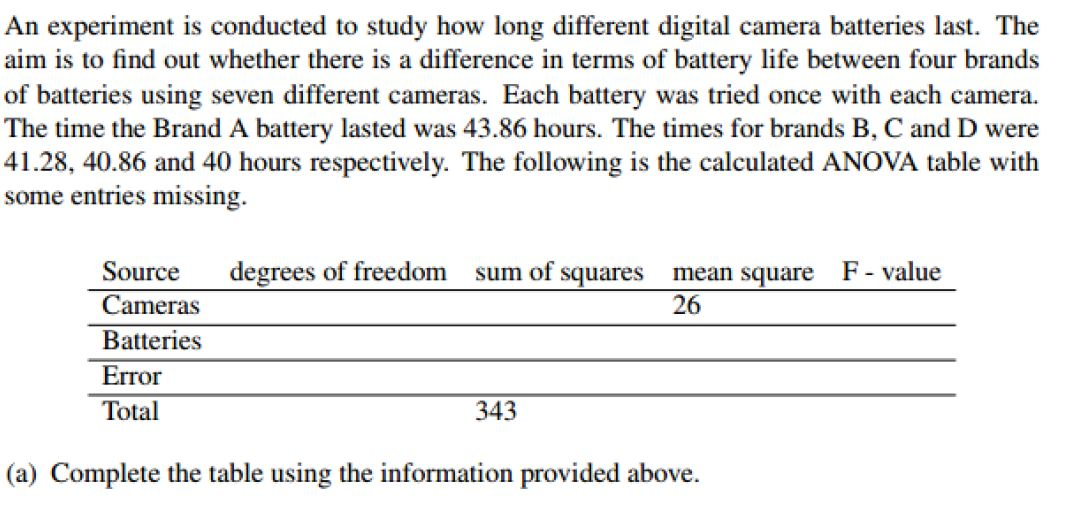
\includegraphics[width=0.9\linewidth]{image/Q28Review1}
	
\end{figure}
\begin{figure}[h!]
	\centering
	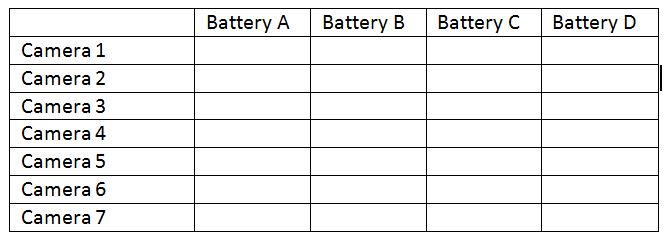
\includegraphics[width=0.9\linewidth]{image/Q28Review3}
	
\end{figure}
\begin{figure}[h!]
	\centering
	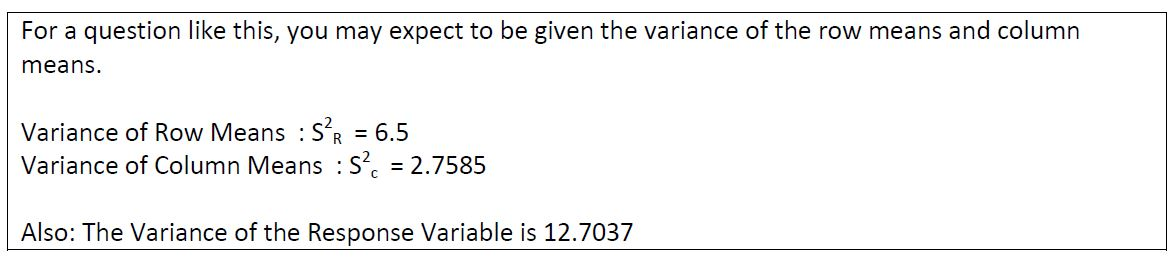
\includegraphics[width=0.9\linewidth]{image/Q28Review2}
	
\end{figure}
\newpage
\subsection*{Q10. Two Way ANOVA (with replicates)}

Consider the following experiment (similar to question 28) where there are 5 measurements per treatment group.
\begin{figure}[h!]
	\centering
	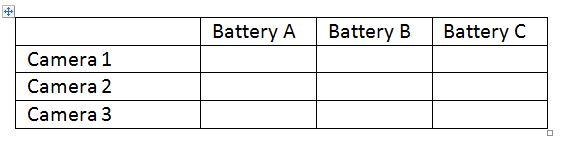
\includegraphics[width=0.8\linewidth]{image/Q29Review}
\end{figure}
Complete the following ANOVA table.\\ \bigskip
\begin{figure}[h!]
	\centering
	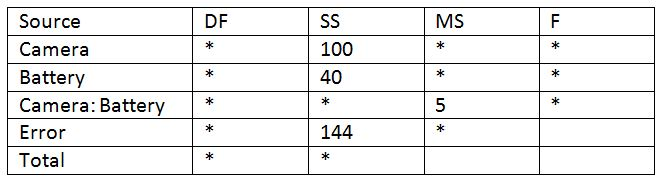
\includegraphics[width=0.8\linewidth]{image/Q29Review2}
\end{figure}\\


For the three F test statistics, state the appropriate degrees of freedom for the corresponding critival value. \textit{(You are not required to perform the hypothesis test)}
\newpage
\subsection*{Q11. Polynomial Regression / Model Selection}

In an experiment to determine hydrolysable tannins in plants by absorption spectroscopy, the following results from ten samples were obtained and are tabulated below. A simple linear regression model, predicting absorbance values using concentration as the independent variable, was fitted to the data.


%%Absorbance= c(0.084, 0.183, 0.326, 0.464, 0.643, 0.707, 0.717, 0.734 ,0.749 ,0.732) ;
%%Concentration= c(0.123, 0.288, 0.562, 0.921, 1.420, 1.717, 1.921, 2.137 ,2.321, 2.467) ;
%%plot(Concentration,Absorbance,pch=18,col="red",font.axis=2,font.lab=2)
%%abline(coef(lm(Absorbance~Concentration)))

%%Conc.Squared = (Concentration^2)
%%Conc.Cubed = (Concentration^3)
%%ModelA = lm(Absorbance~Concentration)
%%ModelB = lm(Absorbance~Concentration+Conc.Squared)
%%ModelC = lm(Absorbance~Concentration+Conc.Squared+Conc.Cubed)

\begin{center}
	\begin{tabular}{|c||c|c|c|c|c|}
		\hline
		%  % after \\: \hline or \cline{col1-col2} \cline{col3-col4} ...
		Sample & 1 & 2 & 3 & 4 & 5 \\ \hline
		Absorbance & 0.084& 0.183& 0.326& 0.464& 0.643\\
		Concentration & 0.123& 0.288& 0.562& 0.921& 1.420\\ \hline
		Sample & 6 & 7 & 8 & 9 & 10 \\ \hline
		Absorbance & 0.707& 0.717& 0.734 &0.749 &0.732\\
		Concentration & 1.717& 1.921& 2.137 &2.321&2.467\\
		\hline
	\end{tabular}
\end{center}

\begin{center}
	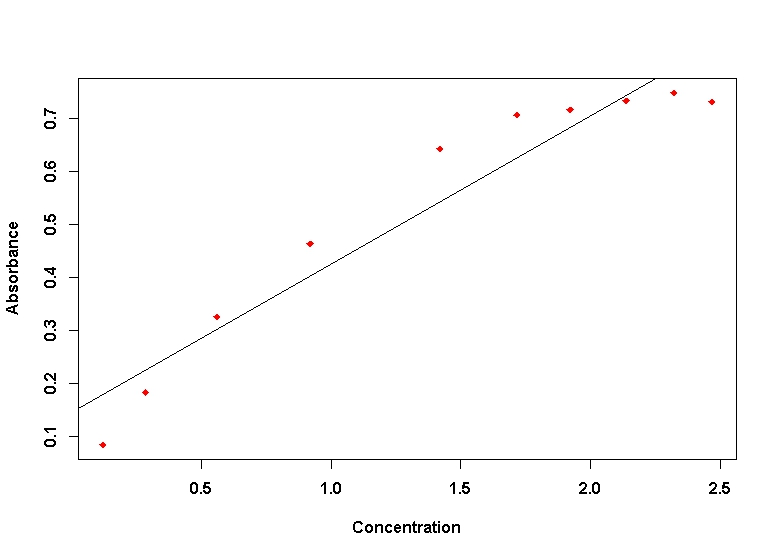
\includegraphics[scale=0.55]{images/ExamQ3plot}
\end{center}

\noindent A Simple Linear regression model and two polynomial models were fitted to the data. Description of all three fitted models are found in the three blocks of \texttt{R} code below. The \emph{Akaike Information Criterion} is listed, for each of the three fitted models.

\begin{itemize}
	\item[i.] (1 marks) Is the simple linear regression model approach suitable for this study? Explain your answer with reference to the scatter-plot.
	\item[ii] (3 marks)  Write down the regression equations of each of the three models.
	
	\item[iv.] (2 marks) Specify which one of the models you would use. Justify your answer with appropriate statistical values.
	
	
	\item[v.] (2 marks) Using the best fit model, predict a value for absorbance when the concentration level is 1.2 $mg/ml$.
\end{itemize}
\newpage
\begin{itemize}
	\begin{framed}
		\item \textbf{Model 1}
		\begin{verbatim}
		> summary(Model1)
		Call:
		lm(formula = Absorb ~ Conc)
		...
		Coefficients:
		Estimate Std. Error t value Pr(>|t|)
		(Intercept)    0.14412    0.04721   3.053   0.0158 *
		Concentration  0.28088    0.02930   9.586 1.16e-05 ***
		...
		
		Residual standard error: 0.07584 on 8 degrees of freedom
		Multiple R-squared: 0.9199,     Adjusted R-squared: 0.9099
		F-statistic: 91.89 on 1 and 8 DF,  p-value: 1.163e-05
		>
		>AIC(Model1)
		[1] -19.4343
		\end{verbatim}
	\end{framed}
	\begin{framed}
		\item \textbf{Model 2}
		\begin{verbatim}
		> summary(Model2)
		Call:
		lm(formula = Absorb ~ Conc + Conc.Squared)
		...
		Coefficients:
		Estimate Std. Error t value Pr(>|t|)
		(Intercept)    0.006582   0.008013   0.821    0.439
		Concentration  0.642935   0.015568  41.299 1.27e-09 ***
		Conc.Squared  -0.140573   0.005894 -23.851 5.79e-08 ***
		...
		Residual standard error: 0.008939 on 7 degrees of freedom
		Multiple R-squared: 0.999,      Adjusted R-squared: 0.9987
		F-statistic:  3592 on 2 and 7 DF,  p-value: 2.879e-11
		>
		> AIC(Model2)
		[1] -61.5338
		\end{verbatim}
	\end{framed}
	\newpage
	
	\begin{framed}
		\item \textbf{Model 3}
		\begin{verbatim}
		> summary(Model3)
		
		Call:
		lm(formula = Absorb ~ Conc+ Conc.Squared + Conc.Cubed)
		...
		...
		Coefficients:
		Estimate Std. Error t value Pr(>|t|)
		(Intercept)    0.013712   0.011629   1.179   0.2830
		Concentration  0.608682   0.042825  14.213 7.58e-06 ***
		Conc.Squared  -0.108186   0.038088  -2.840   0.0296 *
		Conc.Cubed    -0.008196   0.009518  -0.861   0.4223
		...
		
		Residual standard error: 0.009109 on 6 degrees of freedom
		Multiple R-squared: 0.9991,     Adjusted R-squared: 0.9987
		F-statistic:  2306 on 3 and 6 DF,  p-value: 1.422e-09
		>
		> AIC(Model3)
		[1] -60.69903
		\end{verbatim}
	\end{framed}
\end{itemize}
\newpage
\newpage
\subsection*{Q12. Model Selection}

\begin{itemize}
	\item Suppose we have 4 predictor variables :$\{ X_1,X_2,X_3,X_4 \} $\item 
Use Forward and Backward Selection to Choose the Optimal set of Predictor Variables, based on the AIC metrics listed for each combination of predictor variables listed below.
\end{itemize}
{
	\large
\begin{center}
\begin{tabular}{||c|c||c|c||}
	\hline Variables  & AIC & Variables & AIC \\ \hline
	\hline    $\{ \emptyset \} $   & 208.75   &  $\{ X_2,X_4 \} $    & 166.97 \\ \hline 
	\phantom{makespace} & \phantom{makespace} & $\{ X_3,X_4 \} $& 164.16\\
	\hline    $\{ X_1 \} $     &  169.30   &    &  \\ 
	\hline    $\{ X_2 \} $     &  190.79   &  $\{ X_1,X_2,X_3 \}$  & 168.40 \\ \hline
	 $\{ X_3 \} $  & 170.20 &$\{ X_1,X_2,X_4 \} $  & 158.01\\ 
	\hline    $\{ X_4 \} $      &  166.02   &   $\{ X_1,X_3,X_4 \} $  & 157.55\\ 
	\hline        &     &    $\{ X_2,X_3,X_4 \} $  & 165.78 \\ 
	\hline    $\{ X_1,X_2 \} $ &  169.61   &     &  \\ 
	\hline    $\{ X_1,X_3 \} $ &  167.14   &   $\{ X_1,X_2,X_3,X_4 \} $&  159.55\\ 
	\hline    $\{ X_1,X_4 \} $ &  156.01   &    &  \\ 
	\hline $\{ X_2,X_3 \} $ & 166.97 &\phantom{makespace}& \phantom{makespace}\\
	\hline
\end{tabular} 
\end{center}
}
\newpage
\subsection*{Q13. Model Selection}
Use Forward and Backward Selection to Choose the Optimal set of Predictor Variables

{
	\large
	\begin{center}
		\begin{tabular}{|c|c|c|c|c|c|c|c||}\hline
			(None)	&	AIC(Fit0)	&	255.4247	&	Mult $R^2$	&	0	&	adj. $R^2$	&	0	\\ \hline
			Acetic	&	 AIC(FitA)	&	246.6389	&	Mult $R^2$	&	0.3019934	&	adj. $R^2$	&	0.2770646	\\ \hline
			H2S	&	 AIC(FitB)	&	232.0245	&	Mult $R^2$	&	0.5711615	&	adj. $R^2$	&	0.5558458	\\ \hline
			Lactic	&	 AIC(FitC)	&	236.8724	&	Mult $R^2$	&	0.4959486	&	adj. $R^2$	&	0.4779468	\\ \hline
			Acetic, H2S  	&	 AIC(Fit1)	&	233.2438	&	Mult $R^2$	&	0.5821773	&	adj. $R^2$	&	0.5512274	\\ \hline
			Acetic,Lactic 	&	 AIC(Fit2)	&	237.3884	&	Mult $R^2$	&	0.5202762	&	adj. $R^2$	&	0.4847411	\\ \hline
			H2S, Lactic	&	 AIC(Fit3)	&	227.7838	&	Mult $R^2$	&	0.6517024	&	adj. $R^2$	&	0.6259025	\\ \hline
			All Three	&	 AIC(FitAll)	&	229.7775	&	Mult $R^2$	&	0.6517747	&	adj. $R^2$	&	0.6115948	\\ \hline
			
		\end{tabular} 
	\end{center}
}

%==========================================================%
\newpage
\subsection*{Q14. Model Selection}

\begin{itemize}
\item Suppose we have 5 predictor variables.
\item Use \textbf{Forward Selection} and \textbf{Backward Selection} to choose the optimal set of Predictor Variables, based on the AIC metric.
\end{itemize}
{
	\large
	\begin{center}
\begin{tabular}{|c|c|c|c|}
	\hline
$\emptyset$	&	200	&	x1,x2,x3	&	74	\\ \hline
\phantom{makespace}
 &	\phantom{makespace}
 	&	x1,x2,x4	&	75	\\ \hline
x1	&	150	&	x1,x2,x5	&	78	\\ \hline
x2	&	170	&	x1,x3,x4	&	72	\\ \hline
x3	&	135	&	x1,x3,x5	&	82	\\ \hline
x4	&	130	&	x1,x4,x5	&	70	\\ \hline
x5	&	140	&	x2,x3,x4	&	80	\\ \hline
&		&	x2,x3,x5	&	82	\\ \hline
x1,x2	&	90	&	x2,x4,x5	&	78	\\ \hline
x1,x3	&	81	&	x3,x4,x5	&	75	\\ \hline
x1,x4	&	84	&	\phantom{makespace}
	&	\phantom{makespace}
		\\ \hline
x1,x5	&	78	&	x1,x2,x3,x4	&	83	\\ \hline
x2,x3	&	87	&	x1,x2,x3,x5	&	130	\\ \hline
x2,x4	&	78	&	x1,x2,x4,x5	&	104	\\ \hline
x2,x5	&	87	&	x1,x3,x4,x5	&	101	\\ \hline
x3,x4	&	85	&	x2,x3,x4,x5	&	89	\\ \hline
x3,x5	&	88	&		&		\\ \hline
x4,x5	&	86	&	x1,x2,x3,x4,x5	&	100	\\ \hline
		\end{tabular} 
	\end{center}
}
%================================================= %
\newpage
\subsection*{Q15. Regression ANOVA}
%-------------------------------End  of Question 2A%
(4 Marks) Complete the following \textit{Analysis of Variance} Table for a simple linear regression model based on the data provided. The required values are indicated by question marks.
\begin{center}
	\begin{tabular}{|c|c|c|c|c|c|} \hline
		& DF & 	Sum Sq &	Mean Sq &	F value &   	Pr($>$F)    \\ \hline
		Regression &  ? &	9160239 &	? &	 ? &	$< 2.2e^{-16}$ \\ \hline
		Error  & 50 &	2134710 &  	?   &            &       \\ \hline
		Total  & ?  &	? &  	?  &            &       \\ \hline
	\end{tabular} 
\end{center}

Once you have completed this table, compute the following
\begin{itemize}
	\item (1 Mark) The Pearson correlation coefficient for the response variable Y and the predictor variable X.\textit{ (You may assume that the Pearson Correlation Coefficient is a positive number.)}
	\item (1 Mark) The sample standard deviation of the response variable Y.
\end{itemize}
\newpage
\subsection*{Q16. Regression ANOVA}
The mercury level of several tests of sea-water from costal areas was determined by atomic-absorption spectrometry. The results obtained are as follows

\begin{figure}[h!]
	\centering
	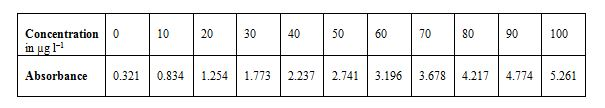
\includegraphics[width=1.1\linewidth]{image/regressionData}
\end{figure}

The analysis of the relationship between concentration and absorbance is obtained in R and presented below. 
\begin{framed}
	\begin{verbatim}
	x<-seq(0,100,by=10)
	y<- c(0.321, 0.834, 1.254, 1.773, 2.237, 2.741, 3.196, 3.678, 
	4.217, 4.774, 5.261)
	model<- lm(y~x)
	summary(model)
	
	Call:
	lm(formula = y ~ x)
	
	Coefficients:
	             Estimate Std. Error t value Pr(>|t|)    
	(Intercept) 0.2933636  0.0234754   12.50 5.45e-07 
	x           0.0491982  0.0003968  123.98 7.34e-16 
	---
	
	Residual standard error: 0.04162 on 9 degrees of freedom
	Multiple R-squared: 0.9994,     Adjusted R-squared: 0.9993 
	F-statistic: 1.537e+04 on 1 and 9 DF,  p-value: 7.337e-16 
	
	confint(model)
	2.5 %     97.5 %
	(Intercept) 0.24025851 0.34646876
	x           0.04830054 0.05009582
	
	\end{verbatim}
\end{framed}

\begin{itemize}
	\item[(i)] (2 marks)
	Determine and interpret the slope and the intercept of the regression line.
	\item[(ii)]  (2 marks) State the 95\% confidence interval for the slope and the intercept coefficients. Interpret this intervals with respect to any relevant hypothesis tests
	\item[(iii)] (2 marks) Explain in which way is the prediction intervals different from the confidence intervals for fitted values in linear regression?
	\item[(iv)] (2 Marks) The following piece of \texttt{R} code gives us a statistical metric. What is this metric? What is it used for? How should it be interpreted.
	
\end{itemize}
\begin{framed}
	\begin{verbatim}
	> AIC(model)
	[1] -34.93389	
	\end{verbatim}
\end{framed}
\newpage

\subsection*{Q17. Regression Models}
\begin{framed}
	\begin{verbatim}
	
	
	> summary(CheesesModel)
	
	Call:
	lm(formula = Taste ~ Acetic + H2S + Lactic)
	
	Residuals:
	Min      1Q  Median      3Q     Max 
	-17.390  -6.612  -1.009   4.908  25.449 
	
	Coefficients:
	            Estimate Std. Error t value Pr(>|t|)   
	(Intercept) -28.8768    19.7354  -1.463  0.15540   
	Acetic        0.3277     4.4598   0.073  0.94198   
	H2S           3.9118     1.2484   3.133  0.00425 **
	Lactic       19.6705     8.6291   2.280  0.03108 * 
	---
	Signif. codes:  0 ‘***’ 0.001 ‘**’ 0.01 ‘*’ 0.05 ‘.’ 0.1 ‘ ’ 1
	
	Residual standard error: 10.13 on 26 degrees of freedom
	Multiple R-squared:  0.6518,    Adjusted R-squared:  0.6116 
	F-statistic: 16.22 on 3 and 26 DF,  p-value: 3.81e-06
	
	\end{verbatim}
\end{framed}
\begin{itemize}
	\item[(i)] (2 marks)
	State the Regression Equation for this model
	\item[(ii)] (8 marks) For each of the regression coefficients, interpret the test for significance. State the null and laternative hypothesis in each case. State your conclusion to each test.
 \item[(iii)] (2 marks) Consider the Code on the next page. State the Regression Equation for this model.
%	\item[(iv)] (2 Marks) The following piece of \texttt{R} code gives us a statistical metric. What is this metric? What is it used for? How should it be interpreted.
	
\end{itemize}

\newpage

<<<<<<< HEAD
\begin{framed}
\begin{verbatim}
> summary(Fit3)

Call:
lm(formula = Taste ~ H2S + Lactic)

Residuals:
Min      1Q  Median      3Q     Max 
-17.343  -6.530  -1.164   4.844  25.618 

Coefficients:
Estimate Std. Error t value Pr(>|t|)   
(Intercept)  -27.592      8.982  -3.072  0.00481 **
H2S            3.946      1.136   3.475  0.00174 **
Lactic        19.887      7.959   2.499  0.01885 * 
---
Signif. codes:  0 ‘***’ 0.001 ‘**’ 0.01 ‘*’ 0.05 ‘.’ 0.1 ‘ ’ 1

Residual standard error: 9.942 on 27 degrees of freedom
Multiple R-squared:  0.6517,    Adjusted R-squared:  0.6259 
F-statistic: 25.26 on 2 and 27 DF,  p-value: 6.551e-07

\end{verbatim}
\end{framed}
=======
\subsection*{Q18. Regression Analysis}
\begin{figure}[h!]
\centering
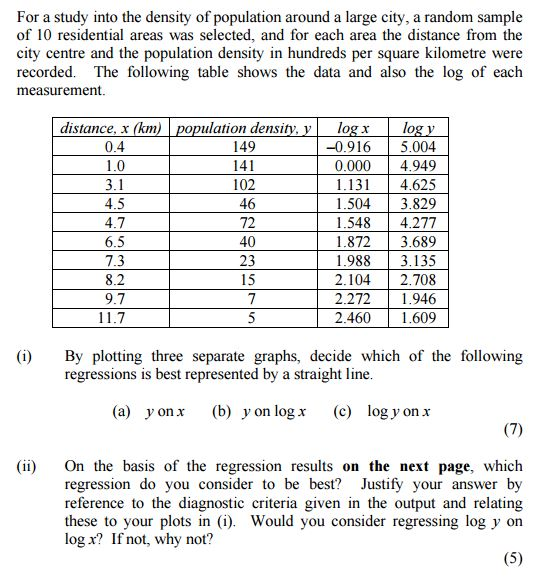
\includegraphics[width=0.8\linewidth]{images/ReviewQ18-a}
\end{figure}
\begin{figure}[h!]
	\centering
	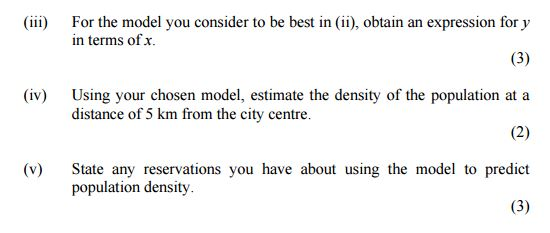
\includegraphics[width=0.8\linewidth]{images/ReviewQ18-b}
\end{figure}
\newpage
\begin{figure}[h!]
	\centering
	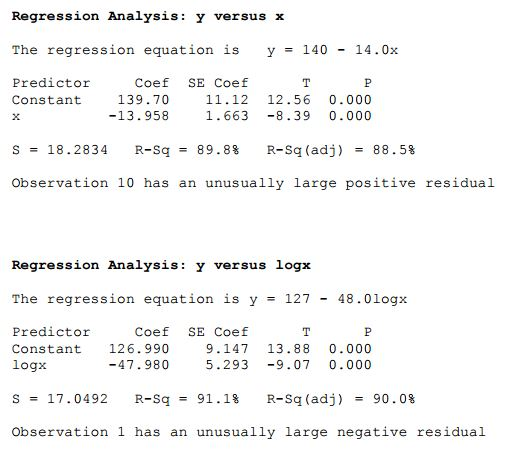
\includegraphics[width=0.8\linewidth]{images/ReviewQ18-c}
\end{figure}
\begin{figure}[h!]
	\centering
	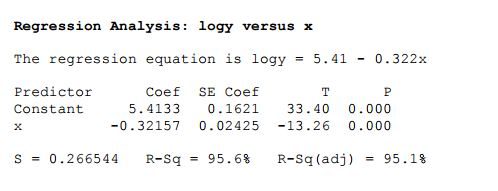
\includegraphics[width=0.8\linewidth]{images/ReviewQ18-d}
\end{figure}


>>>>>>> origin/master
\end{document}